% Created by tikzDevice version 0.12.6 on 2026-05-14 20:37:48
% !TEX encoding = UTF-8 Unicode
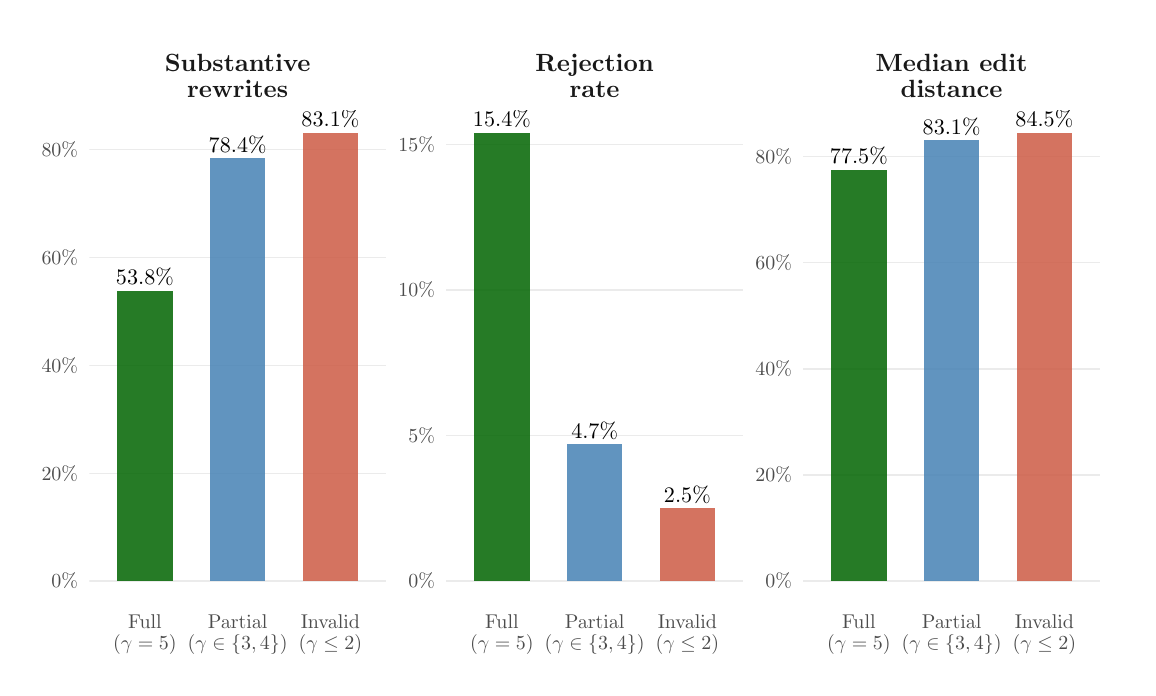
\begin{tikzpicture}[x=1pt,y=1pt]
\definecolor{fillColor}{RGB}{255,255,255}
\path[use as bounding box,fill=fillColor,fill opacity=0.00] (0,0) rectangle (397.48,231.26);
\begin{scope}
\path[clip] (  0.00,  0.00) rectangle (397.48,231.26);
\definecolor{fillColor}{RGB}{255,255,255}

\path[fill=fillColor] (  0.00,  0.00) rectangle (397.48,231.26);
\end{scope}
\begin{scope}
\path[clip] ( 22.25, 23.18) rectangle (129.49,201.38);
\definecolor{drawColor}{gray}{0.92}

\path[draw=drawColor,line width= 0.5pt,line join=round] ( 22.25, 31.28) --
	(129.49, 31.28);

\path[draw=drawColor,line width= 0.5pt,line join=round] ( 22.25, 70.27) --
	(129.49, 70.27);

\path[draw=drawColor,line width= 0.5pt,line join=round] ( 22.25,109.26) --
	(129.49,109.26);

\path[draw=drawColor,line width= 0.5pt,line join=round] ( 22.25,148.25) --
	(129.49,148.25);

\path[draw=drawColor,line width= 0.5pt,line join=round] ( 22.25,187.24) --
	(129.49,187.24);
\definecolor{fillColor}{RGB}{0,100,0}

\path[fill=fillColor,fill opacity=0.85] ( 32.30, 31.28) rectangle ( 52.41,136.16);
\definecolor{fillColor}{RGB}{70,130,180}

\path[fill=fillColor,fill opacity=0.85] ( 65.82, 31.28) rectangle ( 85.93,184.12);
\definecolor{fillColor}{RGB}{205,91,69}

\path[fill=fillColor,fill opacity=0.85] ( 99.33, 31.28) rectangle (119.44,193.28);
\definecolor{drawColor}{RGB}{0,0,0}

\node[text=drawColor,anchor=base,inner sep=0pt, outer sep=0pt, scale=  0.80] at ( 42.36,138.36) {53.8\%};

\node[text=drawColor,anchor=base,inner sep=0pt, outer sep=0pt, scale=  0.80] at ( 75.87,186.32) {78.4\%};

\node[text=drawColor,anchor=base,inner sep=0pt, outer sep=0pt, scale=  0.80] at (109.39,195.48) {83.1\%};
\end{scope}
\begin{scope}
\path[clip] (151.24, 23.18) rectangle (258.49,201.38);
\definecolor{drawColor}{gray}{0.92}

\path[draw=drawColor,line width= 0.5pt,line join=round] (151.24, 31.28) --
	(258.49, 31.28);

\path[draw=drawColor,line width= 0.5pt,line join=round] (151.24, 83.88) --
	(258.49, 83.88);

\path[draw=drawColor,line width= 0.5pt,line join=round] (151.24,136.48) --
	(258.49,136.48);

\path[draw=drawColor,line width= 0.5pt,line join=round] (151.24,189.08) --
	(258.49,189.08);
\definecolor{fillColor}{RGB}{0,100,0}

\path[fill=fillColor,fill opacity=0.85] (161.30, 31.28) rectangle (181.41,193.28);
\definecolor{fillColor}{RGB}{70,130,180}

\path[fill=fillColor,fill opacity=0.85] (194.81, 31.28) rectangle (214.92, 80.73);
\definecolor{fillColor}{RGB}{205,91,69}

\path[fill=fillColor,fill opacity=0.85] (228.33, 31.28) rectangle (248.44, 57.58);
\definecolor{drawColor}{RGB}{0,0,0}

\node[text=drawColor,anchor=base,inner sep=0pt, outer sep=0pt, scale=  0.80] at (171.35,195.48) {15.4\%};

\node[text=drawColor,anchor=base,inner sep=0pt, outer sep=0pt, scale=  0.80] at (204.87, 82.92) {4.7\%};

\node[text=drawColor,anchor=base,inner sep=0pt, outer sep=0pt, scale=  0.80] at (238.38, 59.78) {2.5\%};
\end{scope}
\begin{scope}
\path[clip] (280.24, 23.18) rectangle (387.48,201.38);
\definecolor{drawColor}{gray}{0.92}

\path[draw=drawColor,line width= 0.5pt,line join=round] (280.24, 31.28) --
	(387.48, 31.28);

\path[draw=drawColor,line width= 0.5pt,line join=round] (280.24, 69.63) --
	(387.48, 69.63);

\path[draw=drawColor,line width= 0.5pt,line join=round] (280.24,107.97) --
	(387.48,107.97);

\path[draw=drawColor,line width= 0.5pt,line join=round] (280.24,146.31) --
	(387.48,146.31);

\path[draw=drawColor,line width= 0.5pt,line join=round] (280.24,184.66) --
	(387.48,184.66);
\definecolor{fillColor}{RGB}{0,100,0}

\path[fill=fillColor,fill opacity=0.85] (290.29, 31.28) rectangle (310.40,179.86);
\definecolor{fillColor}{RGB}{70,130,180}

\path[fill=fillColor,fill opacity=0.85] (323.81, 31.28) rectangle (343.92,190.60);
\definecolor{fillColor}{RGB}{205,91,69}

\path[fill=fillColor,fill opacity=0.85] (357.32, 31.28) rectangle (377.43,193.28);
\definecolor{drawColor}{RGB}{0,0,0}

\node[text=drawColor,anchor=base,inner sep=0pt, outer sep=0pt, scale=  0.80] at (300.35,182.06) {77.5\%};

\node[text=drawColor,anchor=base,inner sep=0pt, outer sep=0pt, scale=  0.80] at (333.86,192.79) {83.1\%};

\node[text=drawColor,anchor=base,inner sep=0pt, outer sep=0pt, scale=  0.80] at (367.38,195.48) {84.5\%};
\end{scope}
\begin{scope}
\path[clip] ( 22.25,201.38) rectangle (129.49,226.26);
\definecolor{drawColor}{gray}{0.10}

\node[text=drawColor,anchor=base,inner sep=0pt, outer sep=0pt, scale=  0.90] at ( 75.87,215.58) {\bfseries Substantive};

\node[text=drawColor,anchor=base,inner sep=0pt, outer sep=0pt, scale=  0.90] at ( 75.87,205.86) {\bfseries rewrites};
\end{scope}
\begin{scope}
\path[clip] (151.24,201.38) rectangle (258.49,226.26);
\definecolor{drawColor}{gray}{0.10}

\node[text=drawColor,anchor=base,inner sep=0pt, outer sep=0pt, scale=  0.90] at (204.87,215.58) {\bfseries Rejection};

\node[text=drawColor,anchor=base,inner sep=0pt, outer sep=0pt, scale=  0.90] at (204.87,205.86) {\bfseries rate};
\end{scope}
\begin{scope}
\path[clip] (280.24,201.38) rectangle (387.48,226.26);
\definecolor{drawColor}{gray}{0.10}

\node[text=drawColor,anchor=base,inner sep=0pt, outer sep=0pt, scale=  0.90] at (333.86,215.58) {\bfseries Median edit};

\node[text=drawColor,anchor=base,inner sep=0pt, outer sep=0pt, scale=  0.90] at (333.86,205.86) {\bfseries distance};
\end{scope}
\begin{scope}
\path[clip] (  0.00,  0.00) rectangle (397.48,231.26);
\definecolor{drawColor}{gray}{0.30}

\node[text=drawColor,anchor=base,inner sep=0pt, outer sep=0pt, scale=  0.72] at ( 42.36, 14.18) {Full};

\node[text=drawColor,anchor=base,inner sep=0pt, outer sep=0pt, scale=  0.72] at ( 42.36,  6.40) {($\gamma=5$)};

\node[text=drawColor,anchor=base,inner sep=0pt, outer sep=0pt, scale=  0.72] at ( 75.87, 14.18) {Partial};

\node[text=drawColor,anchor=base,inner sep=0pt, outer sep=0pt, scale=  0.72] at ( 75.87,  6.40) {($\gamma \in \{3,4\}$)};

\node[text=drawColor,anchor=base,inner sep=0pt, outer sep=0pt, scale=  0.72] at (109.39, 14.18) {Invalid};

\node[text=drawColor,anchor=base,inner sep=0pt, outer sep=0pt, scale=  0.72] at (109.39,  6.40) {($\gamma \leq 2$)};
\end{scope}
\begin{scope}
\path[clip] (  0.00,  0.00) rectangle (397.48,231.26);
\definecolor{drawColor}{gray}{0.30}

\node[text=drawColor,anchor=base,inner sep=0pt, outer sep=0pt, scale=  0.72] at (171.35, 14.18) {Full};

\node[text=drawColor,anchor=base,inner sep=0pt, outer sep=0pt, scale=  0.72] at (171.35,  6.40) {($\gamma=5$)};

\node[text=drawColor,anchor=base,inner sep=0pt, outer sep=0pt, scale=  0.72] at (204.87, 14.18) {Partial};

\node[text=drawColor,anchor=base,inner sep=0pt, outer sep=0pt, scale=  0.72] at (204.87,  6.40) {($\gamma \in \{3,4\}$)};

\node[text=drawColor,anchor=base,inner sep=0pt, outer sep=0pt, scale=  0.72] at (238.38, 14.18) {Invalid};

\node[text=drawColor,anchor=base,inner sep=0pt, outer sep=0pt, scale=  0.72] at (238.38,  6.40) {($\gamma \leq 2$)};
\end{scope}
\begin{scope}
\path[clip] (  0.00,  0.00) rectangle (397.48,231.26);
\definecolor{drawColor}{gray}{0.30}

\node[text=drawColor,anchor=base,inner sep=0pt, outer sep=0pt, scale=  0.72] at (300.35, 14.18) {Full};

\node[text=drawColor,anchor=base,inner sep=0pt, outer sep=0pt, scale=  0.72] at (300.35,  6.40) {($\gamma=5$)};

\node[text=drawColor,anchor=base,inner sep=0pt, outer sep=0pt, scale=  0.72] at (333.86, 14.18) {Partial};

\node[text=drawColor,anchor=base,inner sep=0pt, outer sep=0pt, scale=  0.72] at (333.86,  6.40) {($\gamma \in \{3,4\}$)};

\node[text=drawColor,anchor=base,inner sep=0pt, outer sep=0pt, scale=  0.72] at (367.38, 14.18) {Invalid};

\node[text=drawColor,anchor=base,inner sep=0pt, outer sep=0pt, scale=  0.72] at (367.38,  6.40) {($\gamma \leq 2$)};
\end{scope}
\begin{scope}
\path[clip] (  0.00,  0.00) rectangle (397.48,231.26);
\definecolor{drawColor}{gray}{0.30}

\node[text=drawColor,anchor=base east,inner sep=0pt, outer sep=0pt, scale=  0.72] at (276.19, 28.81) {0\%};

\node[text=drawColor,anchor=base east,inner sep=0pt, outer sep=0pt, scale=  0.72] at (276.19, 67.15) {20\%};

\node[text=drawColor,anchor=base east,inner sep=0pt, outer sep=0pt, scale=  0.72] at (276.19,105.49) {40\%};

\node[text=drawColor,anchor=base east,inner sep=0pt, outer sep=0pt, scale=  0.72] at (276.19,143.83) {60\%};

\node[text=drawColor,anchor=base east,inner sep=0pt, outer sep=0pt, scale=  0.72] at (276.19,182.18) {80\%};
\end{scope}
\begin{scope}
\path[clip] (  0.00,  0.00) rectangle (397.48,231.26);
\definecolor{drawColor}{gray}{0.30}

\node[text=drawColor,anchor=base east,inner sep=0pt, outer sep=0pt, scale=  0.72] at (147.19, 28.81) {0\%};

\node[text=drawColor,anchor=base east,inner sep=0pt, outer sep=0pt, scale=  0.72] at (147.19, 81.40) {5\%};

\node[text=drawColor,anchor=base east,inner sep=0pt, outer sep=0pt, scale=  0.72] at (147.19,134.00) {10\%};

\node[text=drawColor,anchor=base east,inner sep=0pt, outer sep=0pt, scale=  0.72] at (147.19,186.60) {15\%};
\end{scope}
\begin{scope}
\path[clip] (  0.00,  0.00) rectangle (397.48,231.26);
\definecolor{drawColor}{gray}{0.30}

\node[text=drawColor,anchor=base east,inner sep=0pt, outer sep=0pt, scale=  0.72] at ( 18.20, 28.81) {0\%};

\node[text=drawColor,anchor=base east,inner sep=0pt, outer sep=0pt, scale=  0.72] at ( 18.20, 67.79) {20\%};

\node[text=drawColor,anchor=base east,inner sep=0pt, outer sep=0pt, scale=  0.72] at ( 18.20,106.78) {40\%};

\node[text=drawColor,anchor=base east,inner sep=0pt, outer sep=0pt, scale=  0.72] at ( 18.20,145.77) {60\%};

\node[text=drawColor,anchor=base east,inner sep=0pt, outer sep=0pt, scale=  0.72] at ( 18.20,184.76) {80\%};
\end{scope}
\end{tikzpicture}
